%% abtex2-modelo-relatorio-tecnico.tex, v<VERSION> laurocesar
%% Copyright 2012-<COPYRIGHT_YEAR> by abnTeX2 group at http://www.abntex.net.br/
%%
%% This work may be distributed and/or modified under the
%% conditions of the LaTeX Project Public License, either version 1.3
%% of this license or (at your option) any later version.
%% The latest version of this license is in
%%   http://www.latex-project.org/lppl.txt
%% and version 1.3 or later is part of all distributions of LaTeX
%% version 2005/12/01 or later.
%%
%% This work has the LPPL maintenance status `maintained'.
%%
%% The Current Maintainer of this work is the abnTeX2 team, led
%% by Lauro César Araujo. Further information are available on
%% http://www.abntex.net.br/
%%
%% This work consists of the files abntex2-modelo-relatorio-tecnico.tex,
%% abntex2-modelo-include-comandos and abntex2-modelo-references.bib
%%

% ------------------------------------------------------------------------
% ------------------------------------------------------------------------
% abnTeX2: Modelo de Relatório Técnico/Acadêmico em conformidade com
% ABNT NBR 10719:2015 Informação e documentação - Relatório técnico e/ou
% científico - Apresentação
% ------------------------------------------------------------------------
% ------------------------------------------------------------------------

\documentclass[
	% -- opções da classe memoir --
	12pt,				% tamanho da fonte
	%openright,			% capítulos começam em pág ímpar (insere página vazia caso preciso)
	oneside,			% twoside para impressão em recto e verso. Oposto a oneside
	a4paper,			% tamanho do papel.
	% -- opções da classe abntex2 --
	%chapter=TITLE,		% títulos de capítulos convertidos em letras maiúsculas
	%section=TITLE,		% títulos de seções convertidos em letras maiúsculas
	%subsection=TITLE,	% títulos de subseções convertidos em letras maiúsculas
	%subsubsection=TITLE,% títulos de subsubseções convertidos em letras maiúsculas
	% -- opções do pacote babel --
	english,			% idioma adicional para hifenização
	brazil,				% o último idioma é o principal do documento
	]{abntex2}


% ---
% PACOTES
% ---

% ---
% Pacotes fundamentais
% ---
\usepackage{lmodern}			% Usa a fonte Latin Modern
\usepackage[T1]{fontenc}		% Selecao de codigos de fonte.
\usepackage[utf8]{inputenc}		% Codificacao do documento (conversão automática dos acentos)
\usepackage{indentfirst}		% Indenta o primeiro parágrafo de cada seção.
\usepackage{color}				% Controle das cores
\usepackage{graphicx}			% Inclusão de gráficos
\usepackage{microtype} 			% para melhorias de justificação
% ---

% ---
% Pacotes adicionais, usados no anexo do modelo de folha de identificação
% ---
\usepackage{multicol}
\usepackage{multirow}
% ---

% ---
% Pacotes adicionais, usados apenas no âmbito do Modelo Canônico do abnteX2
% ---
\usepackage{lipsum}				% para geração de dummy text
% ---

% ---
% Pacotes de citações
% ---
\usepackage[brazilian,hyperpageref]{backref}	 % Paginas com as citações na bibl
\usepackage[alf]{abntex2cite}	% Citações padrão ABNT

% ---
% Pacote de gráficos
% ---
% \usepackage{tikz}

% ---
% Pacote para adicionar facilmente quebra de linha em células das tabelas
% ---
\usepackage{makecell}

% ---
% Pacote para melhorar a aparência das tabelas e permitir formatação complexa
% ---
\usepackage{booktabs}

% ---
% Pacote para permitir tabelas ocuparem múltiplas páginas (cuidado com Overleaf gratuito)
% ---
\usepackage{longtable}

% ---
% Pacote para controlar formatação das legendas
% ---
\usepackage{caption}
\captionsetup[longtable]{font=normalsize,singlelinecheck=false,justification=raggedright,position=top}

% ---
% Pacote para manter as tabelas dentro das seções em que foram criadas
% ---
\usepackage[section]{placeins}

% ---
% Pacote para controlar floats, não usar em conjunto com o pacote float comum
% ---
% \usepackage{floatrow}
% \floatsetup[longtable]{LTcapwidth=table}

% ---
% CONFIGURAÇÕES DE PACOTES
% ---

% ---
% Configurações do pacote backref
% Usado sem a opção hyperpageref de backref
\renewcommand{\backrefpagesname}{Citado na(s) página(s):~}
% Texto padrão antes do número das páginas
\renewcommand{\backref}{}
% Define os textos da citação
\renewcommand*{\backrefalt}[4]{
	\ifcase #1 %
		Nenhuma citação no texto.%
	\or
		Citado na página #2.%
	\else
		Citado #1 vezes nas páginas #2.%
	\fi}%
% ---

% ---
% Configurações do pacote tikz
% ---
% \usetikzlibrary{shapes.geometric, arrows.meta, positioning}

% ---
% Informações de dados para CAPA e FOLHA DE ROSTO
% ---
\titulo{NotoriousNote \\ \huge{Visão do Projeto}}
\autor{Equipe EmptyCoffeeCups \\ Davi Antônio da Silva Santos \and Marcos Adriano \and Jonathan Jorge Barbosa Oliveira \and Wellington Jonathan}
\local{Brasília, Distrito Federal, Brasil}
\data{2021, v2021.04.19}
\instituicao{%
  Universidade de Brasília -- UnB
  \par
  Faculdade do Gama -- FGA
}
\tipotrabalho{Relatório técnico}
% O preambulo deve conter o tipo do trabalho, o objetivo,
% o nome da instituição e a área de concentração
\preambulo{Documento de visão e planejamento do projeto NotoriousNote.}
% ---

% ---
% Configurações de aparência do PDF final

% alterando o aspecto da cor azul
\definecolor{blue}{RGB}{41,5,195}

% informações do PDF
\makeatletter
\hypersetup{
     	%pagebackref=true,
		pdftitle={\@title},
		pdfauthor={\@author},
    	pdfsubject={\imprimirpreambulo},
	    pdfcreator={LaTeX with abnTeX2},
		pdfkeywords={abnt}{latex}{abntex}{abntex2}{relatório técnico},
		colorlinks=true,       		% false: boxed links; true: colored links
    	linkcolor=blue,          	% color of internal links
    	citecolor=blue,        		% color of links to bibliography
    	filecolor=magenta,      		% color of file links
		urlcolor=blue,
		bookmarksdepth=4
}
\makeatother
% ---

% ---
% Espaçamentos entre linhas e parágrafos
% ---

% O tamanho do parágrafo é dado por:
\setlength{\parindent}{1.3cm}

% Controle do espaçamento entre um parágrafo e outro:
\setlength{\parskip}{0.2cm}  % tente também \onelineskip

% ---
% compila o indice
% ---
\makeindex
% ---

% ----
% Início do documento
% ----
\begin{document}

% Seleciona o idioma do documento (conforme pacotes do babel)
%\selectlanguage{english}
\selectlanguage{brazil}

% Retira espaço extra obsoleto entre as frases.
\frenchspacing

% ----------------------------------------------------------
% ELEMENTOS PRÉ-TEXTUAIS
% ----------------------------------------------------------
% \pretextual

% ---
% Capa
% ---
\imprimircapa
% ---

% ---
% Folha de rosto
% (o * indica que haverá a ficha bibliográfica)
% ---
\imprimirfolhaderosto*
% ---

% ---
% Anverso da folha de rosto:
% ---

% {
% \ABNTEXchapterfont

% \vspace*{\fill}

% Conforme a ABNT NBR 10719:2015, seção 4.2.1.1.1, o anverso da folha de rosto
% deve conter:

% \begin{alineas}
%   \item nome do órgão ou entidade responsável que solicitou ou gerou o
%   relatório;
%   \item título do projeto, programa ou plano que o relatório está relacionado;
%   \item título do relatório;
%   \item subtítulo, se houver, deve ser precedido de dois pontos, evidenciando a
%   sua subordinação ao título. O relatório em vários volumes deve ter um título
%   geral. Além deste, cada volume pode ter um título específico;
%   \item número do volume, se houver mais de um, deve constar em cada folha de
%   rosto a especificação do respectivo volume, em algarismo arábico;
%   \item código de identificação, se houver, recomenda-se que seja formado
%   pela sigla da instituição, indicação da categoria do relatório, data,
%   indicação do assunto e número sequencial do relatório na série;
%   \item classificação de segurança. Todos os órgãos, privados ou públicos, que
%   desenvolvam pesquisa de interesse nacional de conteúdo sigiloso, devem
%     informar a classificação adequada, conforme a legislação em vigor;
%   \item nome do autor ou autor-entidade. O título e a qualificação ou a função
%   do autor podem ser incluídos, pois servem para indicar sua autoridade no
%   assunto. Caso a instituição que solicitou o relatório seja a mesma que o
%   gerou, suprime-se o nome da instituição no campo de autoria;
%   \item local (cidade) da instituição responsável e/ou solicitante; NOTA: No
%   caso de cidades homônimas, recomenda-se o acréscimo da sigla da unidade da
%   federação.
%   \item ano de publicação, de acordo com o calendário universal (gregoriano),
%   deve ser apresentado em algarismos arábicos.
% \end{alineas}

% \vspace*{\fill}
% }

% ---
% Agradecimentos
% ---
% \begin{agradecimentos}
% O agradecimento principal é direcionado a Youssef Cherem, autor do
% \nameref{formulado-identificacao} (\autopageref{formulado-identificacao}).

% Os agradecimentos especiais são direcionados ao Centro de Pesquisa em
% Arquitetura da Informação\footnote{\url{http://www.cpai.unb.br/}} da Universidade de
% Brasília (CPAI), ao grupo de usuários
% \emph{latex-br}\footnote{\url{http://groups.google.com/group/latex-br}} e aos
% novos voluntários do grupo
% \emph{\abnTeX}\footnote{\url{http://groups.google.com/group/abntex2} e
% \url{http://www.abntex.net.br/}}~que contribuíram e que ainda
% contribuirão para a evolução do abn\TeX.

% \end{agradecimentos}
% ---

% ---
% RESUMO
% ---

% resumo na língua vernácula (obrigatório)
% \setlength{\absparsep}{18pt} % ajusta o espaçamento dos parágrafos do resumo
% \begin{resumo}
%  Segundo a \citeonline[3.1-3.2]{NBR6028:2003}, o resumo deve ressaltar o
%  objetivo, o método, os resultados e as conclusões do documento. A ordem e a extensão
%  destes itens dependem do tipo de resumo (informativo ou indicativo) e do
%  tratamento que cada item recebe no documento original. O resumo deve ser
%  precedido da referência do documento, com exceção do resumo inserido no
%  próprio documento. (\ldots) As palavras-chave devem figurar logo abaixo do
%  resumo, antecedidas da expressão Palavras-chave:, separadas entre si por
%  ponto e finalizadas também por ponto.

%  \noindent
%  \textbf{Palavras-chaves}: latex. abntex. editoração de texto.
% \end{resumo}
% ---

% Histórico de revisão
\chapter*[Histórico de Revisões]{Histórico de Revisões}

\IBGEtabfontsize
\begin{longtable}{@{}p{0.1\textwidth}p{0.1\textwidth}p{0.6\textwidth}p{0.1\textwidth}@{}}
%\caption{}
%\label{} \\
\toprule
\textbf{Data} & \textbf{Versão} & \textbf{Descrição} & \textbf{Autor} \\ \midrule \endhead
18/02/2021 & 2021.02.18 & Versão inicial & Equipe EmptyCoffeCups \\ \hline
09/03/2021 & 2021.03.11 & \begin{tabular}{@{}p{0.6\textwidth}@{}}Renomear projeto de Notório para NotoriousNote\\Remoção do excesso de páginas em branco\\Modificação da declaração do problema\\Modificação dos objetivos de projeto, aumentando o escopo deste\\Modificação no escopo do MVP\\Acreéscimo do professor na organização do projeto\\Remoção do prazo estimado nas ferramentas de hardware e software\\Clarificação da escalabilidade dos problemas\\Adequação da matriz de comunicação às práticas do projeto\\Acréscimo dos itens dos \textit{backlogs}\\Atualizar versões das ferramentas de software \end{tabular} & Equipe EmptyCoffeCups \\ \midrule
25/03/2021 & 2021.03.25-preview & \begin{tabular}{@{}p{0.6\textwidth}@{}}Remover US02 e US17\\Mudar descrição da US08, US09, US13, US18, US20 e US21\\Estabelecer pontos para as histórias de usuário normalizados a partir de US01\\Remover funcionalidade de exportar notas em texto puro e requisito não funcional de suporte a APIs Android do MVP\\Remover funcionalidade FT02\\Mudar título da US07 e US13\\Mudar título das funcionalidades FT01 e FT04\\Especificar APIs do Android suportadas no NFR01 \end{tabular} & Equipe EmptyCoffeCups \\ \midrule
27/03/2021 & 2021.03-27-preview & \begin{tabular}{@{}p{0.6\textwidth}@{}}Adicionar às dependências o pacote Flutter sqflite na versão \^{}2.0.0+3\\Atualizar Android Studio da versão 4.1.2 para 4.1.3\\Atualizar Flutter da versão 2.0.1 para 2.0.3\\Atualizar Dart da versão 2.12.0 para 2.12.2\\Atualizar Kotlin da versão 1.4.30 para 1.4.31\\Atualizar Gradle da versão 4.1.2 para 4.1.3\\Atualizar extensão do Android Studio Flutter da versão 54.0.1 para 54.1.1\\Atualizar extensão do Android Studio Kotlin da versão 1.4.30 para 1.4.31\\Atualizar dependência Android Firebase BoM da versão 26.5.0 para 26.6.0\\Atualizar pacote Flutter firebase\_auth da versão 0.20+1 para \^{}1.0.1\\Atualizar pacote Flutter firebase\_core da versão 0.7.0 para \^{}1.0.2\\Atualizar pacote Flutter cloud\_firestore da versão 0.16.0 para \^{}1.0.3\\Atualizar pacote Flutter provider da versão 4.3.3 para \^{}5.0.0\\Reorganizar ordem das dependências na tabela\\Configurar tabela do histórico de revisões para ser apresentada em múltiplas páginas\end{tabular} & Davi Antônio da Silva Santos\\ \midrule
01/04/2021 & 2021.04.01 & \begin{tabular}{@{}p{0.6\textwidth}@{}}Atualizar dependência Android Firebase BoM da versão 26.6.0 para 26.8.0\\Separar objetivos do projeto em primários e secundários\\Substituir temas de investimento por temas estratégicos (SAFe 5.0)\\Mudar sigla dos temas estratégicos de IT para ST\\Atualizar descrição do tema estratégico ST01 (IT01)\\Atualizar descrição do épico EP01\\Alterar descrição da funcionalidade FT05\\Retirar geração de APK da \textit{sprint} 2 no cronograma, pois não aconteceu\\Substituir configuração do Firebase para configuração do ambiente e movê-la da \textit{sprint} 2 para a  3\\Especificar que o APK gerado na \textit{sprint} 3 apenas testa a configuração do ambiente\\Melhorar a clareza na descrição do problema\\Priorização das histórias com MoSCoW\\Correção de erros gramaticais na descrição das histórias\\Ajustes de leiaute no documento\\Criar, pontuar e priorizar histórias US22, US23, US24 e US25\end{tabular} & Equipe EmptyCoffeCups \\ \midrule
15/04/2021 & 2021.04.15-preview & \begin{tabular}{@{}p{0.6\textwidth}@{}}Atualizar Flutter da versão 2.0.3 para 2.0.4\\Atualizar extensão do Android Studio Flutter da versão 54.1.1 para 55.1.1\\Atualizar extensão do Android Studio Kotlin da versão 1.4.31 para 1.4.32\\Separação do trabalho em abordagem ágil e tradicional \\ Escrita das necessidades \\ Elicitação dos requisitos funcionais \end{tabular} & Equipe EmptyCoffeCups \\ \midrule
19/04/2021 & 2021.04.19 & \begin{tabular}{@{}p{0.6\textwidth}@{}}Alterar descrição do RF21\\Criar tabelas de requisitos e casos de uso\\Adicionar diagrama de casos de uso do sistema\\Adicionar RF23\\Adicionar ferramenta de compilação Android SDK Build Tools na versão 30.0.3\\Criar lista de ilustrações\end{tabular} & Equipe EmptyCoffeCups \\ \midrule
 & & & \\ \bottomrule
\end{longtable}
\cleardoublepage

% ---
% inserir lista de ilustrações
% ---
\pdfbookmark[0]{\listfigurename}{lof}
\listoffigures*
\cleardoublepage
% ---

% ---
% inserir lista de tabelas
% ---
\pdfbookmark[0]{\listtablename}{lot}
\listoftables*
\cleardoublepage
% ---

% ---
% inserir lista de abreviaturas e siglas
% ---
\begin{siglas}
  \item[API] \foreignlanguage{english}{\textit{Application Programming Interface}}
  \item[BD] Banco de Dados
  \item[BLoC] \foreignlanguage{english}{\textit{Business Logic of Component}}
  \item[DB] \foreignlanguage{english}{\textit{Database}}
  \item[IDE] \foreignlanguage{english}{\textit{Integrated Development Environment}}
  \item[SAFe] \foreignlanguage{english}{\textit{Scaled Agile Framework}}
  \item[SDK] \foreignlanguage{english}{\textit{Software Development Kit}}
  \item[SOLID] \foreignlanguage{english}{\textit{Single responsibility, Open-closed, Liskov substitution, Interface segregation, Dependency inversion}}
  \item[UI] \foreignlanguage{english}{\textit{User Interface}}
  \item[UnB] Universidade de Brasília
\end{siglas}
% ---

% ---
% inserir lista de símbolos
% ---
% \begin{simbolos}
%   \item[$ \Gamma $] Letra grega Gama
%   \item[$ \Lambda $] Lambda
%   \item[$ \zeta $] Letra grega minúscula zeta
%   \item[$ \in $] Pertence
% \end{simbolos}
% ---

% ---
% inserir o sumario
% ---
\pdfbookmark[0]{\contentsname}{toc}
\tableofcontents*
\cleardoublepage
% ---


% ----------------------------------------------------------
% ELEMENTOS TEXTUAIS
% ----------------------------------------------------------
\textual
%[Este artefato deve ser utilizado como guia para o registro das informações gerais do projeto. Deve ser refinado e atualizado ao longo do projeto].

\chapter{Introdução}
%\section{Problema}

\section{Declaração do Problema}
%[Forneça uma declaração resumindo o problema que está sendo resolvido por este projeto. O seguinte formato pode ser usado:]

\begin{table}[ht]
\IBGEtab{%
\caption{Declaração do problema}%
\label{tab:declaracao_problema}%
}{%
\begin{tabular}{@{}p{0.29\textwidth}p{0.7\textwidth}@{}}
\toprule
% descreva o problema
O problema & grande quantidade de atividades simultâneas exigidas pela sociedade atual \\ \midrule
% informe as partes interessadas afetadas pelo problema
Afeta & pessoas que possuem dificuldade em organizar seus compromissos caso não os anotem \\ \midrule
% qual é o impacto desse problema?
Cujo impacto é & risco de não cumprimento de compromissos e desorganização das tarefas individuais \\ \midrule
% liste alguns benefícios principais de uma solução de sucesso
Uma solução de sucesso seria & permitir que os criem anotações com a possibilidade de configurar lembretes para notificar anotações específicas, criem anotações para lista de tarefas, classifiquem anotações por grupos, realizem backups remotos e locais das anotações \\ \bottomrule
\end{tabular}%
}{%\fonte{}%
}
\end{table}

\section{Objetivos do Projeto}
%[Forneça o objetivo principal do projeto, e objetivos secundários (caso haja)]
\subsection{Objetivos primários}
Criar uma aplicação que permita o usuário crie anotações, listas de tarefa, lembretes para as anotações. Também deve ser possível ao usuário acessar \textit{templates} de anotações para criar modelos comuns mais rapidamente.

\subsection{Objetivos secundários}
A aplicação também deve ser capaz de exportar os dados de suas notas e listas de tarefas para formatos que podem ser importados em outros aplicativos ou armazenados em dispositivos externos: JSON, \texttt{org-mode} e texto puro. Além disso, também deve ser possível fazer o backup dos dados do dispositivo na nuvem e compartilhar a informação com outros aplicativos usando funções nativas do sistema operacional móvel.

\chapter{\foreignlanguage{english}{\textit{Stakeholders}}}
% [Forneça a lista de stakeholders envolvidos no projeto]

\begin{table}[ht]
\IBGEtab{%
\caption{Lista das partes interessadas (\textit{stakeholders}) envolvidas no projeto}%
\label{tab:stakeholders}%
}{%
\begin{tabular}{@{}p{0.2\textwidth}p{0.25\textwidth}p{0.5\textwidth}@{}}
\toprule
\textbf{Nome} & \textbf{Descrição} & \textbf{Responsabilidades} \\ \midrule
% Nomeie o tipo de parte interessada & Descreva resumidamente a parte interessada & Resuma as principais responsabilidades das partes interessadas com relação ao sistema que está sendo desenvolvido; \\ ou seja, seu interesse como parte interessada. Por exemplo, esta parte interessada:\\ garante que o sistema será sustentável\\ garante que haverá uma demanda de mercado para as características do produto\\ monitora o progresso do projeto\\ aprova financiamento\\ e assim por diante
Professor orientador & Professor da disciplina de Requisitos de Software & \makecell[c{p{0.5\textwidth}}]{Monitora o progresso do projeto \\ Auxilia na validação e verificação de requisitos} \\ \midrule
Desenvolvedores & Alunos da disciplina de Requisitos de Software & \makecell[c{p{0.5\textwidth}}]{Elicitam, analisam, especificam, validam, verificam e gerenciam requisitos\\ Desenvolvem e testam o software \\ Produzem um software utilizável} \\ \midrule
Usuário & Pessoas que utilizarão o aplicativo & \makecell[c{p{0.5\textwidth}}]{Utilizar a aplicação móvel\\ Reportar problemas aos desenvolvedores} \\ \bottomrule
\end{tabular}%
}{%\fonte{}%
}
\end{table}

\chapter{Visão Geral do Produto}

\section{Declaração de Posição do Produto}
%[Forneça uma declaração geral resumindo, no nível mais alto, a posição exclusiva que o produto pretende preencher no mercado. Uma declaração de posição do produto comunica a intenção da aplicação e a importância do projeto para todo o pessoal envolvido. O seguinte formato pode ser usado:]

\begin{table}[ht]
\IBGEtab{%
\caption{Declaração de posição do produto.}%
\label{tab:declaracao_posicao_prodututo}%
}{%
\begin{tabular}{@{}p{0.2\textwidth}p{0.8\textwidth}@{}}
\toprule
% cliente alvo
\textbf{Para} & usuários de \textit{smartphone} Android \\ \midrule
% declaração da necessidade ou oportunidade
\textbf{Quem} & usuários que queiram controle sobre as suas notas escritas em um celular, mas não querem abandonar a comodidade de armazenarem seus dados na nuvem \\ \midrule
% O [nome do produto] & é um/uma [categoria do produto]
\textbf{O NotoriousNote} & é uma aplicação móvel de registro de notas \\ \midrule
% declaração do principal benefício; ou seja, a razão convincente para comprar, utilizar, etc.
\textbf{Que} & permite que o usuário exporte os dados da própria aplicação, de modo que possa armazená-los em outro lugar com o objetivo de, por exemplo, realizar backup de notas importantes \\ \hline
% alternativa competitiva primária
\textbf{Ao contrário} & do Google Keep, que dificulta a exportação das notas e listas de tarefas feitas no próprio aplicativo \\ \midrule
% declaração de diferenciação primária
\textbf{Nosso produto} & permite que o usuário exporte os seus dados em um formato legíveis (JSON, texto puro e \texttt{org-mode}) que podem ser usado em outras aplicações \\ \bottomrule
\end{tabular}%
}{%\fonte{}%
}
\end{table}

\section{Mínimo Produto Viável (MVP)}
%[Forneça uma lista de características mínimas que o produto deve possuir para que possa ser lançado]
\begin{itemize}
    % \item Aplicação deve ser executável em sistemas operacionais móveis Android com suporte as APIs 24 a 30;
    \item Criar, apagar, editar e visualizar de notas de texto com título e conteúdo;
    \item Criar, apagar, editar e visualizar etiquetas;
    \item Atribuir etiquetas a uma anotação;
    % \item Exportar notas e listas de tarefas em texto puro;
    \item Visualizar notas por etiquetas específicas.
    % \item Criação de listas de tarefa com título e tarefas que podem ser registradas como terminadas ou não;
    % \item Capacidade de salvar notas e listas de tarefa em nuvem (Cloud Firestore);
    % \item Capacidade de exportar notas e listas de tarefas em JSON;
    % \item Capacidade de ler notas e listas de tarefas salvas localmente em JSON.
\end{itemize}

\chapter{Visão Geral do Projeto}
\section{Organização do Projeto}
%[apresentada a divisão de atribuições e responsabilidades entre os membros do projeto, sem qualquer relação de hierarquia ou grau de importância. Todos os integrantes são igualmente importantes e responsáveis pelo sucesso do projeto.]
A organização do projeto seguirá a divisão de papéis proposta pelo \textit{framework} Scrum \cite{scrum_guide}.

\begin{table}[ht]
\IBGEtab{%
\caption{Organização do projeto}%
\label{tab:organizacao_projeto}%
}{%
\begin{tabular}{@{}p{0.2\textwidth}p{0.24\textwidth}p{0.24\textwidth}p{0.24\textwidth}@{}}
\toprule
\textbf{Papel} & \textbf{Atribuições} & \textbf{Responsável} & \textbf{Participantes} \\ \midrule
Desenvolvedor & \makecell[c{p{0.24\textwidth}}]{Membro da equipe ágil\\Execução das disciplinas de Engenharia de Software} & Jonathan Jorge, \foreignlanguage{english}{Wellington} Jonathan & Davi Antônio, Jonathan Jorge, Marcos Adriano, Wellington Jonathan\\ \midrule
Scrum Master & Responsável pelo cumprimento da metodologia de desenvolvimento Scrum & Marcos Adriano & - \\ \midrule
Product Owner & Responsável por manter o conceito das funcionalidades e melhorias, de forma que sigam a visão definida para o produto ou projeto. & Davi Antônio & - \\ \midrule
Professor Orientador & Professor da disciplina de Requisitos de Software & Professor Dr. Marsicano & Professor Dr. Marsicano \\ \bottomrule
\end{tabular}%
}{%\fonte{}%
}
\end{table}

\chapter{Ferramentas, Ambiente e Infraestrutura}
\section{Hardware}
% [Esta seção apresenta a infra-estrutura de hardware adequada para o desenvolvimento do projeto.]
% [Exemplo:

\begin{table}[ht]
\IBGEtab{%
\caption{Infraestrutura de hardware necessária}%
\label{tab:infra_hardware}%
}{%
\begin{tabular}{@{}p{0.14\textwidth}p{0.14\textwidth}p{0.27\textwidth}p{0.05\textwidth}p{0.2\textwidth}@{}}
\toprule
\textbf{Perfil} & \textbf{Tipo} & \textbf{Configurações} & \textbf{Qtd.} & \textbf{Observação} \\ \midrule
Desenvolvedor & Computador & \makecell[c{p{0.27\textwidth}}]{Interface USB \\ Mínimo 8 GiB RAM \\ Resolução de tela mínima 1280x800 px.} & 04 & - \\ \bottomrule
\end{tabular}%
}{%\fonte{}%
}
\end{table}
\newpage%
\section{Software}
%[Esta seção apresenta a infra-estrutura de software adequada para o desenvolvimento do projeto.]
%[Exemplo:
\begin{table}[ht]
\caption{Infraestrutura de software necessária}%
\label{tab:ambiente_software}
\centering
\IBGEtabfontsize
\begin{tabular}{@{}p{0.125\textwidth}p{0.145\textwidth}p{0.145\textwidth}p{0.135\textwidth}p{0.100\textwidth}p{0.115\textwidth}@{}}
\toprule
\textbf{Perfil} & \textbf{Tipo} & \textbf{Nome} & \textbf{Versão} & \textbf{Licenças}  & \textbf{Observação} \\ \midrule
Todos & Controle de Versão & Git & 2.25.1 ou superior & 04  & - \\ \midrule
Todos & IDE & Android Studio & 4.1.3 & 04  & - \\ \midrule
Todos & SDK & Flutter & 2.0.4 & 04  & - \\ \midrule
Todos & Linguagem de programação & Dart & 2.12.2 & 04  & - \\ \midrule
Todos & Linguagem de programação & Kotlin & 1.4.32 & 04  & - \\ \midrule
Todos & Extensão do Android Studio & Dart & 201.9335 & 04  & - \\ \midrule
Todos & Extensão do Android Studio & Flutter & 55.1.1 & 04  & - \\ \midrule
Todos & Extensão do Android Studio & Kotlin & 1.4.31-release-Studio4.1-1 & 04  & - \\ \midrule
Todos & Pacote Flutter & provider & \^{}5.0.0 & 04 & - \\ \midrule
Todos & Pacote Flutter & sqflite & \^{}2.0.0+3 & 04 & - \\ \midrule
Todos & Pacote Flutter & firebase\_core & \^{}1.0.2 & 04 & - \\ \midrule
Todos & Pacote Flutter & firebase\_auth & \^{}1.0.1 & 04  & - \\ \midrule
Todos & Pacote Flutter & cloud\_firestore & \^{}1.0.3 & 04  & - \\ \midrule
Todos & Dependência Android & google-services & 4.3.5 & 04  & - \\ \midrule
Todos & Dependência Android & firebase-bom & 26.8.0 & 04  & - \\ \midrule
Todos & Ferramenta de compilação & gradle & 4.1.3 & 04  & - \\ \midrule
Todos & Ferramenta de compilação & Android SDK Build Tools & 30.0.3 & 04  & - \\ \bottomrule
\end{tabular}%
\end{table}

\chapter{Processo de Gerência de Projeto}
\section{Planejamento das Fases e Iterações do Projeto}
% [Registrar o projeto, as fases de seu ciclo de vida e suas iterações, especificando suas datas de início e de fim, bem como os produtos a serem gerados.]

\begin{table}[ht]
\IBGEtab{%
\caption{Planejamento de gerência de projeto}%
\label{tab:fases_iteracoes}%
}{% p{0.14\textwidth} %\makecell[c{p{0.27\textwidth}}]{}
\begin{tabular}{@{}llll@{}}
\toprule
\textbf{Sprint} & \textbf{Início} & \textbf{Fim} & \textbf{Incrementos Esperados} \\ \midrule
1 & 02/02 & 18/02 & \makecell{Atividades da unidade 1 \\ Sugestão de ideia de projeto \\ Primeira versão do documento de visão} \\ \midrule
2 & 23/02 & 11/03 & \makecell{Atividades da unidade 2 \\ Atualização do documento de visão} \\ \midrule
3 & 16/03 & 01/04 & \makecell{Atividades da unidade 3 \\ Atualização do documento de visão \\ Configuração do ambiente de desenvolvimento \\ Geração do primeiro APK em modo \textit{debug} para testar ambiente} \\ \midrule
4 & 06/04 & 22/04 & \makecell{Atividades da unidade 4 \\ Atualização do documento de visão \\ Geração do segundo APK em modo \textit{debug}} \\ \midrule
5 & 27/04 & 13/05 & \makecell{Atividades da unidade 5 \\ Geração da APK otimizada para lançamento \\ Entrega da versão final do documento de visão} \\ \bottomrule
\end{tabular}%
}{%\fonte{}%
}
\end{table}

\section{Processo de Desenvolvimento e Mensuração}
% [Especifique como será acompanhado o progresso, por exemplo, por meio de reuniões de revisão diárias, avaliações de iteração, relatórios de Burndown de Projeto e Burndown de Iteração.]
A equipe utilizará o \textit{framework} Scrum, com utilização reuniões semanais no lugar da \textit{daily} e com retrospectiva da \textit{sprint}, para gerenciar o projeto. O progresso será acompanhado usando-se um quadro Kanban na plataforma Github, a qual também atua como repositório remoto para o sistema de versionamento distribuído Git, que será utilizado para o controle de versão do código fonte.

Os requisitos do projeto serão separados em histórias de usuário e estas serão transformadas em cartões de um quadro Kanban que corresponderá ao \textit{backlog} do projeto usando-se o sistema de \textit{issues} disponibilizado pela plataforma.

Através da reunião de planejamento serão escolhidas as \textit{issues} do quadro de \textit{backlog} do produto que serão movidas para o \textit{backlog} de cada \textit{sprint}. Cada quadro possui colunas geradas a partir de etiquetas que identificam o estado da \textit{issue}: \textit{backlog} da \textit{sprint}, a fazer, fazendo, testando e feito.

Um cartão será movido para a coluna a fazer assim que tiver um responsável atribuído; de a fazer para a coluna fazendo quando trabalho de codificação iniciar-se; de fazendo para testando enquanto é validado e de testando para pronto após a aprovação do Product Owner e do Professor Orientador na cerimônia de Revisão da \textit{Sprint}.

A equipe acompanhará o desempenho atribuindo a cada história no \textit{backlog} do produto uma pontuação. Essa pontuação será atribuída pela equipe nas reuniões de planejamento usando-se a técnica de \textit{Planning Poker} \cite{planning_poker} usando a sequência de Fibonacci. Os pontos serão atribuídos após a discussão do grupo, e podem ser reatribuídos caso se considere que a atribuição inicial esteja desbalanceada.

Para permitir um acompanhamento mais próximo do desenvolvimento, estimando a capacidade de desenvolvimento da equipe, será usada a métrica \textit{velocity} para cada iteração, a qual consiste no número de pontos de histórias executadas com sucesso numa dada \textit{sprint}. Caso aconteça uma mudança nos valores de pontos das histórias a métrica terá que ser recalculada.

% \section{\foreignlanguage{english}{\textit{Milestones}} e Objetivos do Projeto}

\section{Matriz de Comunicação}
A comunicação do grupo é feita principalmente pelo Telegram e por reuniões no Microsoft Teams.
%[Esta seção descreve a estratégia de comunicação adotada para monitoramento do progresso do projeto. Identificar a periodicidade de reuniões e o envio dos relatórios exigidos pelo processo e opcionalmente outros relatórios exigidos pelo cliente.]

\begin{table}[ht]
\IBGEtab{%
\caption{Matriz de comunicação}%
\label{tab:matriz_comunicacao}%
}{%
\begin{tabular}{@{}p{0.25\textwidth}p{0.25\textwidth}p{0.2\textwidth}p{0.25\textwidth}@{}}
\toprule
\textbf{Descrição} & \textbf{Área/Envolvidos} & \textbf{Periodicidade} & \textbf{Produtos Gerados} \\ \midrule
% \multirow{2}{=}{\begin{tabular}[c]{@{}p{0.25\textwidth}@{}}- Acompanhamento das Atividades em Andamento\\ - Acompanhamento dos Riscos, Compromissos, Ações Pendentes, Indicadores \end{tabular}} & - Equipe do Projeto & - Semanal & \multirow{2}{=}{\begin{tabular}[c]{@{}p{0.2\textwidth}@{}}- Ata de reunião\\ - Relatório de situação do projeto \end{tabular}} \\ \cmidrule(lr){2-3}
%  &  & - Quinzenal &  \\ & & & \\ & & & \\ & & & \\ & & & \\ \midrule



- Comunicar situação do projeto & \begin{tabular}[c]{@{}l@{}}- Equipe \\ - Professor\end{tabular} & - Semanal & \begin{tabular}[c]{@{}p{0.25\textwidth}@{}}- Comunicação com o Professor Orientador\\- Atualizações nos \foreignlanguage{english}{\textit{backlogs}} \end{tabular} \\ \midrule

- Comunicar situação entre membros(\textit{Sprint Planning}) & \begin{tabular}[c]{@{}l@{}}- Equipe \\ \end{tabular} & - No inicio da Sprint & \begin{tabular}[c]{@{}p{0.25\textwidth}@{}}-  \textit{Product Backlog} da \textit{Sprint} \\  \end{tabular} \\ \midrule

% - Comunicar situação entre membros(\textit{daily}) & \begin{tabular}[c]{@{}l@{}}- Equipe \\ \end{tabular} & - Seg , Quar e Sex & - \\ \midrule



- Comunicar situação entre membros(\textit{Sprint Review}) & \begin{tabular}[c]{@{}l@{}}- Equipe \\ \end{tabular} & - No final da \textit{Sprint} & \begin{tabular}[c]{@{}p{0.25\textwidth}@{}}-  \\  \end{tabular} \\ \midrule




- Comunicar situação entre membros (\textit{Sprint Retrospective}) & \begin{tabular}[c]{@{}l@{}}- Equipe \\ \end{tabular} & - No final da \textit{Sprint} & \begin{tabular}[c]{@{}p{0.25\textwidth}@{}}- Atualizações nos documentos de visão e nos \foreignlanguage{english}{\textit{backlogs}} \\  \end{tabular} \\ \bottomrule



\end{tabular}%
}{%\fonte{}%
}
\end{table}

\section{Escalabilidade do Projeto}

Com o andamento do projeto, previsivelmente ocorreram conflitos que devem ser identificados o mais breve possível, e que devem ser imediatamente solucionados. O tratamento desses conflitos deve ser algo orgânico do fluxo de desenvolvimento de software, e ter antecipadamente para diferentes problemas subsequentes frentes de resolução, sendo que nem todo conflito pode ou deve ser solucionado em uma primeira instancia.

O fluxo do projeto deve ter em seu acompanhamento um monitoramento continuo de revisão e correção. Deve-se garantir quando encontrados conflitos esses devem ser imediatamente tratados com prioridade para o \textit{Scrum Master} e escalonados, caso seja necessário, ao Professor Orientador para sua dada resolução, evitando o comprometimento do fluxo de projeto.

Quando tratado o \textit{backlog}, todo conflito deve ser mensurado e verificado de antemão com o \textit{Product Owner}, se houver problemas na resolução, a situação será levada para o Professor Orientador, assim como conflitos que põem em risco o projeto.

\section{Gerenciamento de Riscos}
O objetivo principal da Gestão de Riscos é controlar  impedimentos de qualquer tipo, que possa surgir durante o ciclo de desenvolvimento , impedindo o progresso do projeto de acordo com as previsões iniciais. Comumente citado no PMBOK também pode ser utilizado em projetos que utilizem metodologias ágeis  assim como o \textit{Scrum}. Dessas forma os riscos elicitados foram os seguintes:
\begin{table}[ht]
\IBGEtab{%
\caption{Lista de riscos}%
\label{tab:lista_riscos}%
}{%
\begin{tabular}{@{}p{0.24\textwidth}p{0.24\textwidth}p{0.24\textwidth}p{0.2\textwidth}@{}}
\toprule
\textbf{Código} & \textbf{Risco} & \textbf{Ação} & \textbf{Nível de Risco} \\ \midrule
RS01 & Não Versionamento do código & Refatoração do código para ser aceito na versão mais recente do projeto. & Médio \\ \midrule
RS02 & Equipe desorganizada & Reunião para alinhar a equipe. & Baixo \\ \midrule
RS03 & Não priorização dos requisitos & Analisar as dependências dos requisitos e priorizar os que há menos dependência & Baixo\\ \midrule
RS04 & Má elicitação dos requisitos & Refazer o requisito e todas as partes que o mesmo está envolvido & Alto \\ \midrule
RS05 & Falta de comunicação da equipe & Reunir para alinhar a equipe & Médio \\ \midrule
RS06 & Não integração do código & Refatoração do código para permitir integração & Médio \\ \midrule
\end{tabular}%
}{%\fonte{}%
}
\end{table}
%[Para o Gerenciamento de Riscos devem ser realizadas tarefas, como:
%\begin{itemize}
%\item
 %   \item Identificar todos os riscos possíveis e detectáveis em cada fase do projeto;
 %   \item Executar as ações para mitigar os riscos que tenham um alto grau de exposição ao risco caso este ocorra na Lista de Riscos do Projeto;
  %  \item Fazer uma revisão da lista dos riscos periodicamente, com o propósito de averiguar uma possível incidência de um risco e ver se há outros riscos ainda não relatados;
   % \item Em caso de confirmação de um risco previsto, agir no sentido de contingenciá-lo conforme programado;%    \item Registrar os riscos no Painel de Controle do Projeto e no Plano do Projeto (Riscos iniciais);]
%\end{itemize}


\section{Critérios de Replanejamento}
%[Descrever os critérios de replanejamento que serão utilizados, caso seja necessário realizá-lo no projeto.]
Será necessário replanejar o projeto caso algumas dessas situações venha acontecer:
\begin{itemize}
    \item Algum integrante ficar impossibilitado de colaborar com o projeto;
    \item Caso o professor considere inadequado o tema;
    \item Caso os requisitos não sejam suficientes para aplicar o conteúdo da unidade curricular.
    \item Caso a tecnologia escolhida torne-se inadequada ao desenvolvimento do projeto.
\end{itemize}

\part{Processo Ágil}

\chapter{Itens dos \textit{Backlogs} SAFe}
Os itens dos \textit{backlogs} foram construídos usando-se a estrutura de requisitos sugerida pelo \foreignlanguage{english}{\textit{Scaled Agile Framework}} (SAFe) em \cite{safe_requirements_model}, temas estratégicos, requisitos não funcionais, épicos, \textit{features} e histórias de usuário.

\section{Temas Estratégicos}
Os temas estratégicos, presentes na tabela \ref{tab:temas_estratégicos}, são responsáveis por estabelecer a perspectiva de negócio e dirigir os épicos que serão gerados no nível de Portfólio.

\begin{table}[ht]
\IBGEtab{%
\caption{Temas estratégicos}%
\label{tab:temas_estratégicos}%
}{%
\begin{tabular}{@{}ll@{}}
\toprule
\textbf{Temas estratégicos} & \textbf{Descrição} \\ \midrule
ST01 & Controle de anotações \\ \bottomrule
\end{tabular}%
}{%\fonte{}%
}
\end{table}

\section{Épicos}
Os épicos descritos na tabela \ref{tab:epicos} estão presentes no \foreignlanguage{english}{\textit{backlog}} do Portfólio, definindo o mínimo produto viável.

\begin{table}[ht]
\IBGEtab{%
\caption{Épicos}%
\label{tab:epicos}%
}{%
\begin{tabular}{@{}ll@{}}
\toprule
\textbf{Épicos} & \textbf{Descrição} \\ \midrule
EP01 & Criar, exportar e organizar anotações\\ \bottomrule
\end{tabular}%
}{%\fonte{}%
}
\end{table}

\section{\textit{Features}}
As \foreignlanguage{english}{\textit{features}} (funcionalidades), presentes na tabela \ref{tab:features}, estão atreladas a um épico e estão localizadas nos \foreignlanguage{english}{\textit{backlogs}} da solução e de programa. Como o projeto não será grande o suficiente, decidiu-se remover o nível de solução.

\begin{table}[htb]
\IBGEtab{%
\caption{\textit{Features}}%
\label{tab:features}%
}{%
\begin{tabular}{@{}lll@{}}
\toprule
\textbf{Épicos} & \textbf{Features} & \textbf{Descrição} \\ \midrule
EP01 & FT01 & Gerência de backup \\ \midrule
EP01 & FT03 & Gerência de anotações \\ \midrule
EP01 & FT04 & Gestão de tempo básica\\ \bottomrule
\end{tabular}%
}{%\fonte{}%
}
\end{table}

\section{Histórias do usuário}
As histórias de usuário (tabela \ref{tab:historias_de_usuario}) são derivadas a partir das \foreignlanguage{english}{\textit{features}} e estão presentes nos \foreignlanguage{english}{\textit{backlogs}} da equipe, de onde são retirados para serem colocados nos quadros \textit{kanban} de cada equipe ágil. Nessa tabela, a coluna ID especifica a identificação única de cada história de usuário e sua pontuação de dificuldade normalizada em relação à US01 seguindo a sequência de Fibonacci.

As tarefas foram priorizadas usando-se a metodologia MoSCoW. Histórias indicadas como \textit{must} são fundamentais para implementação do MVP e são mandatórias, histórias \textit{could} podem ser retiradas do MVP sem grande impacto, as histórias \textit{should} podem ser retiradas sem problema e as \textit{will not have} não são importantes para o período de tempo atual.

\IBGEtabfontsize
\begin{longtable}{@{}p{0.1\textwidth}p{0.05\textwidth}p{0.29\textwidth}p{0.39\textwidth}p{0.1\textwidth}@{}}
\caption{Histórias de usuário}
\label{tab:historias_de_usuario} \\
\toprule
\textbf{Feature} & \textbf{ID} & \textbf{Nome} & \textbf{Descrição} & \textbf{MSCW} \\ \midrule
FT01 & US10 (2) & Criar conta & Eu como usuário desejo criar conta para utilizar o armazenamento remoto & C\\ \midrule
FT01 & US11 (8) & Configurar preferências de armazenamento e backup & Eu como usuário desejo configurar preferências de armazenamento e backup para salvar minhas anotações remotamente e localmente ou apenas localmente & C\\ \midrule
FT01 & US12 (13) & Sincronizar anotações locais com armazenamento remoto (nuvem) & Eu como usuário desejo sincronizar anotações locais com armazenamento remoto (nuvem) para não perder minhas anotações em caso de roubo & C\\ \midrule
FT01 & US09 (5) & Exportar anotações em armazenamento local & Eu como usuário desejo exportar anotações em armazenamento local para compartilhar por outras aplicações ou manter uma cópia de segurança & C\\ \midrule
FT01 & US20 (8) & Restaurar anotações a partir de arquivo de backup & Eu como usuário desejo recuperar anotações a partir de um arquivo de backup para que não seja necessário reescrevê-las manualmente & C\\ \midrule
FT03 & US01 (1*) & Criar anotações & Eu como usuário desejo criar anotações para lembrar de conteúdos que me interessem & M\\ \midrule
% FT03 & US02 (3) & Salvar anotações & Eu como usuário desejo salvar anotações para poder consultar seus conteúdos posteriormente &\\ \midrule
FT03 & US03 (1) & Visualizar anotações & Eu como usuário desejo visualizar anotações para visualizar as que já foram criadas & M\\ \midrule
FT03 & US04 (2) & Editar anotações & Eu como usuário desejo editar anotações para que possa alterar seus conteúdos sem que seja necessário reescrevê-los completamente & M\\ \midrule
FT03]& US05 (2) & Deletar anotações & Eu como usuário desejo deletar anotações para remover conteúdos que não são mais necessários & M\\ \midrule
FT03 & US06 (3) & Etiquetar anotações & Eu como usuário desejo etiquetar anotações para organizá-las & M\\ \midrule
FT03 & US07 (3) & Agrupar anotações por etiquetas & Eu como usuário desejo agrupar anotações por etiquetas para visualizar apenas as anotações com as etiquetadas selecionadas & S\\ \midrule
FT03 & US13 (8) & Criar listas de tarefas & Eu como usuário desejo criar listas de tarefas para organizar mais facilmente minhas tarefas e saber quais restam ser feitas & S\\ \midrule
FT03 & US14 (8) & Consultar anotações & Eu como usuário desejo consultar anotações por conteúdo para facilmente acessar algo que preciso lembrar & S\\ \midrule
FT03 & US15 (5) & Arquivar anotações & Eu como usuário desejo arquivar anotações para ocultá-las da visualização principal sem que seja necessário excluí-las & S\\ \midrule
% FT03 & US17 & Habilitar colaboração em anotações & Eu como usuário desejo habilitar colaboração em anotações para poder ter a colaboração de outros usuários nas minhas anotações &\\ \midrule
FT03 & US18 (8) & Compartilhar anotações com outros aplicativos & Eu como usuário desejo compartilhar anotações para poder utilizá-las em outros aplicativos & C\\ \midrule
FT03 & US21 (21) & Relatório do tempo de execução de tarefas e notas temporizadas & Eu como usuário desejo criar relatório do tempo de execução de tarefas e anotações temporizadas para poder visualizar o tempo gasto & W\\ \midrule
FT03 & US22 (5) & Criar etiquetas & Eu como usuário desejo criar etiquetas para organizar minhas anotações & M\\ \midrule
FT03 & US23 (5) & Editar etiquetas & Eu como usuário desejo editar etiquetas para não precisar criar outra etiqueta & M\\ \midrule
FT03 & US24 (8) & Deletar etiquetas & Eu como usuário desejo deletar etiquetas para remover as que não são mais necessárias & M\\ \midrule
FT03 & US25 (5) & Visualizar etiquetas & Eu como usuário desejo visualizar etiquetas para ver quais etiquetas eu já criei & M\\ \midrule
FT04 & US08 (5) & Verificar tempo de duração de uma anotação & Eu como usuário desejo que seja possível especificar a data de término de um lembrete para a anotação especificada usando tempo relativo ao início para que não seja necessário especificar tempo absoluto na data de término & W\\ \midrule
FT04 & US16 (21) & Configurar alarmes & Eu como usuário desejo configurar lembretes nas anotações para poder ser alertado por eles & W\\ \midrule
FT04 & US19 (8) & Cronometrar tempo de execução de tarefas em listas & Eu como usuário desejo cronometrar tempo de execução de tarefas listadas em uma anotação para saber o tempo gasto & W\\ \bottomrule
\end{longtable}

\section{Requisitos não funcionais}
\begin{table}[ht]
\IBGEtab{%
\caption{Requisitos não funcionais}%
\label{tab:requisitos_nao_funcionais}%
}{%
\begin{tabular}{@{}ll@{}}
\toprule
\textbf{ID} & \textbf{Descrição} \\ \midrule
NFR01 & Compatibilidade com Android 7 a 11 (APIs 24 a 30) \\ \bottomrule
\end{tabular}%
}{%\fonte{}%
}
\end{table}

\part{Abordagem Tradicional - Processo Unificado }


\chapter{Engenharia de Requisitos - Abordagem tradicional}
\section{Necessidades}

\IBGEtabfontsize
\begin{longtable}{@{}p{0.05\textwidth}p{0.2\textwidth}p{0.05\textwidth}p{0.2\textwidth}p{0.2\textwidth}p{0.2\textwidth}@{}}
\caption{Necessidades}
\label{tab:necessidades} \\
\toprule
\textbf{Id.} & \textbf{Necessidade} & \textbf{Prioridade} & \textbf{Problema} & \textbf{Solução Atual} & \textbf{Solução Proposta} \\ \midrule
N1 & Gerenciar anotações & Alta & Dificuldade em organizar múltiplos compromissos de forma eficiente & Gerenciamento dos compromissos em blocos adesivos ou agenda física & Digitalização do processo de registro e gestão das anotações \\ \midrule
N2 & Cópia de segurança das anotações & Média & Ter acesso às anotações sempre que precisar, mesmo em caso de roubos e perdas & Não é realizado backup das anotações & Digitalizar as anotações possibilitará a cópia eficiente das anotações \\ \midrule
N3 &Lembrar compromissos & Média & Recordar dos compromissos de forma simples e eficiente & A lembrança dos compromissos é feita analisando a agenda e anotações periodicamente & Elaboração de um sistema que alerta o usuário dos seus lembretes \\ \bottomrule
\end{longtable}

\section{Requisitos funcionais}
\IBGEtabfontsize
\begin{longtable}{@{}p{0.05\textwidth}p{0.95\textwidth}@{}}
\caption{Requisitos}
\label{tab:requisitos} \\
\toprule
\textbf{Id.} & \textbf{Descrição} \\ \midrule
RF1 & Para criar uma anotação o usuário deve sinalizar que quer criá-la e fornecer um título ou um conteúdo \\ \midrule
RF2 & Para ler anotações é necessário que existam anotações criadas \\ \midrule
RF3 & Ao modificar anotação o usuário deve selecionar uma anotação criada e alterar o campo do título ou conteúdo   \\ \midrule
RF4 & Para apagar anotações o usuário deve selecionar uma anotação existente e confirmar que deseja apagá-la. \\ \midrule

RF5 & Para criar etiquetas o usuário deve sinalizar que quer criá-la e fornecer um nome. \\ \midrule
RF6 & Para ler etiquetas o usuário deve selecionar uma etiqueta existente \\ \midrule
RF7 & Para modificar etiquetas o usuário deve selecionar uma etiqueta que já exista e modificar o seu conteúdo \\ \midrule
RF8 & Para apagar etiquetas deve ser selecionada, pelo usuário, uma etiqueta existente, e essa ação de apagar deve ser confirmada para que se realize \\ \midrule
RF9 & Para atribuir etiquetas o usuário deve selecionar uma anotação e uma etiqueta existente \\ \midrule

RF10 & Para realizar uma cópia de segurança na nuvem o usuário deve acessar uma conta já existente, caso não tiver é necessário criar uma nova conta  \\ \midrule

RF11 & Após ter criado a conta o usuário deve confirmar seu e-mail para que sua conta seja validada\\ \midrule

RF12 & Para criar uma lista de tarefas o usuário deve sinalizar que quer criá-la e fornecer um título \\ \midrule
RF13 & Para ler uma lista de tarefas é necessário que existam listas de tarefas criadas \\ \midrule
RF14 & Para modificar uma lista de tarefas o usuário deve selecionar uma lista criada e alterar o campo do título \\ \midrule
RF15 & Para apagar listas de tarefas o usuário deve selecionar uma existente e confirmar que deseja apagá-la \\ \midrule

RF16 & Para criar uma tarefa o usuário deve sinalizar que quer criá-la e fornecer um conteúdo \\ \midrule
RF17 & Para ler uma tarefa é necessário que esta exista \\ \midrule
RF18 & Para modificar uma tarefa o usuário deve selecionar uma tarefa e alterar os campos de conteúdo ou de conclusão da tarefa \\ \midrule
RF19 & Para apagar listas de tarefas o usuário deve selecionar uma existente e confirmar que deseja apagá-la \\ \midrule
RF20 & O sistema deve encaminhar alerta quando um lembrete for acionado. \\ \midrule
RF21 & Para um usuário criar um lembrete ele deve sinalizar que quer criá-lo em uma tarefa e configurar os horários que deseja ser notificado\\ \midrule
RF22 & O usuário pode cronometrar o tempo gasto para executar uma tarefa, que corresponde ao período de tempo entre a criação  e a marcação da tarefa como concluída \\\midrule
RF23 & Apos a criação da conta o usuário pode gerenciar a mesma, podendo alterar a senha e e-mail\\\bottomrule
\end{longtable}

\section{Casos de uso}

\IBGEtabfontsize
\begin{longtable}{@{}ll@{}}
\caption{Relação entre requisitos e casos de uso}
\label{tab:requisitos_x_casos_de_uso} \\
\toprule
\textbf{Requisitos} & \textbf{Casos de Uso} \\ \midrule
 RF01, RF02, RF03, RF04 & Gerência de Anotações\\ \midrule
 RF01 ,RF05, RF06, RF07, RF08, RF09 & Gerência de Etiquetas\\ \midrule
 RF012, RF13, RF14, RF15, RF16, RF17, RF18, RF19, RF21, RF22 & Gerência de Tarefas\\ \midrule
 RF10 & Gerência de Backup\\ \midrule
 RF10, RF11, RF23 & Gerência de Conta\\ \midrule
 RF21, RF22 & Gerência de Notificações\\ \bottomrule

\end{longtable}

\section{Diagrama de casos de uso}
\begin{figure}[htb]
    \centering
    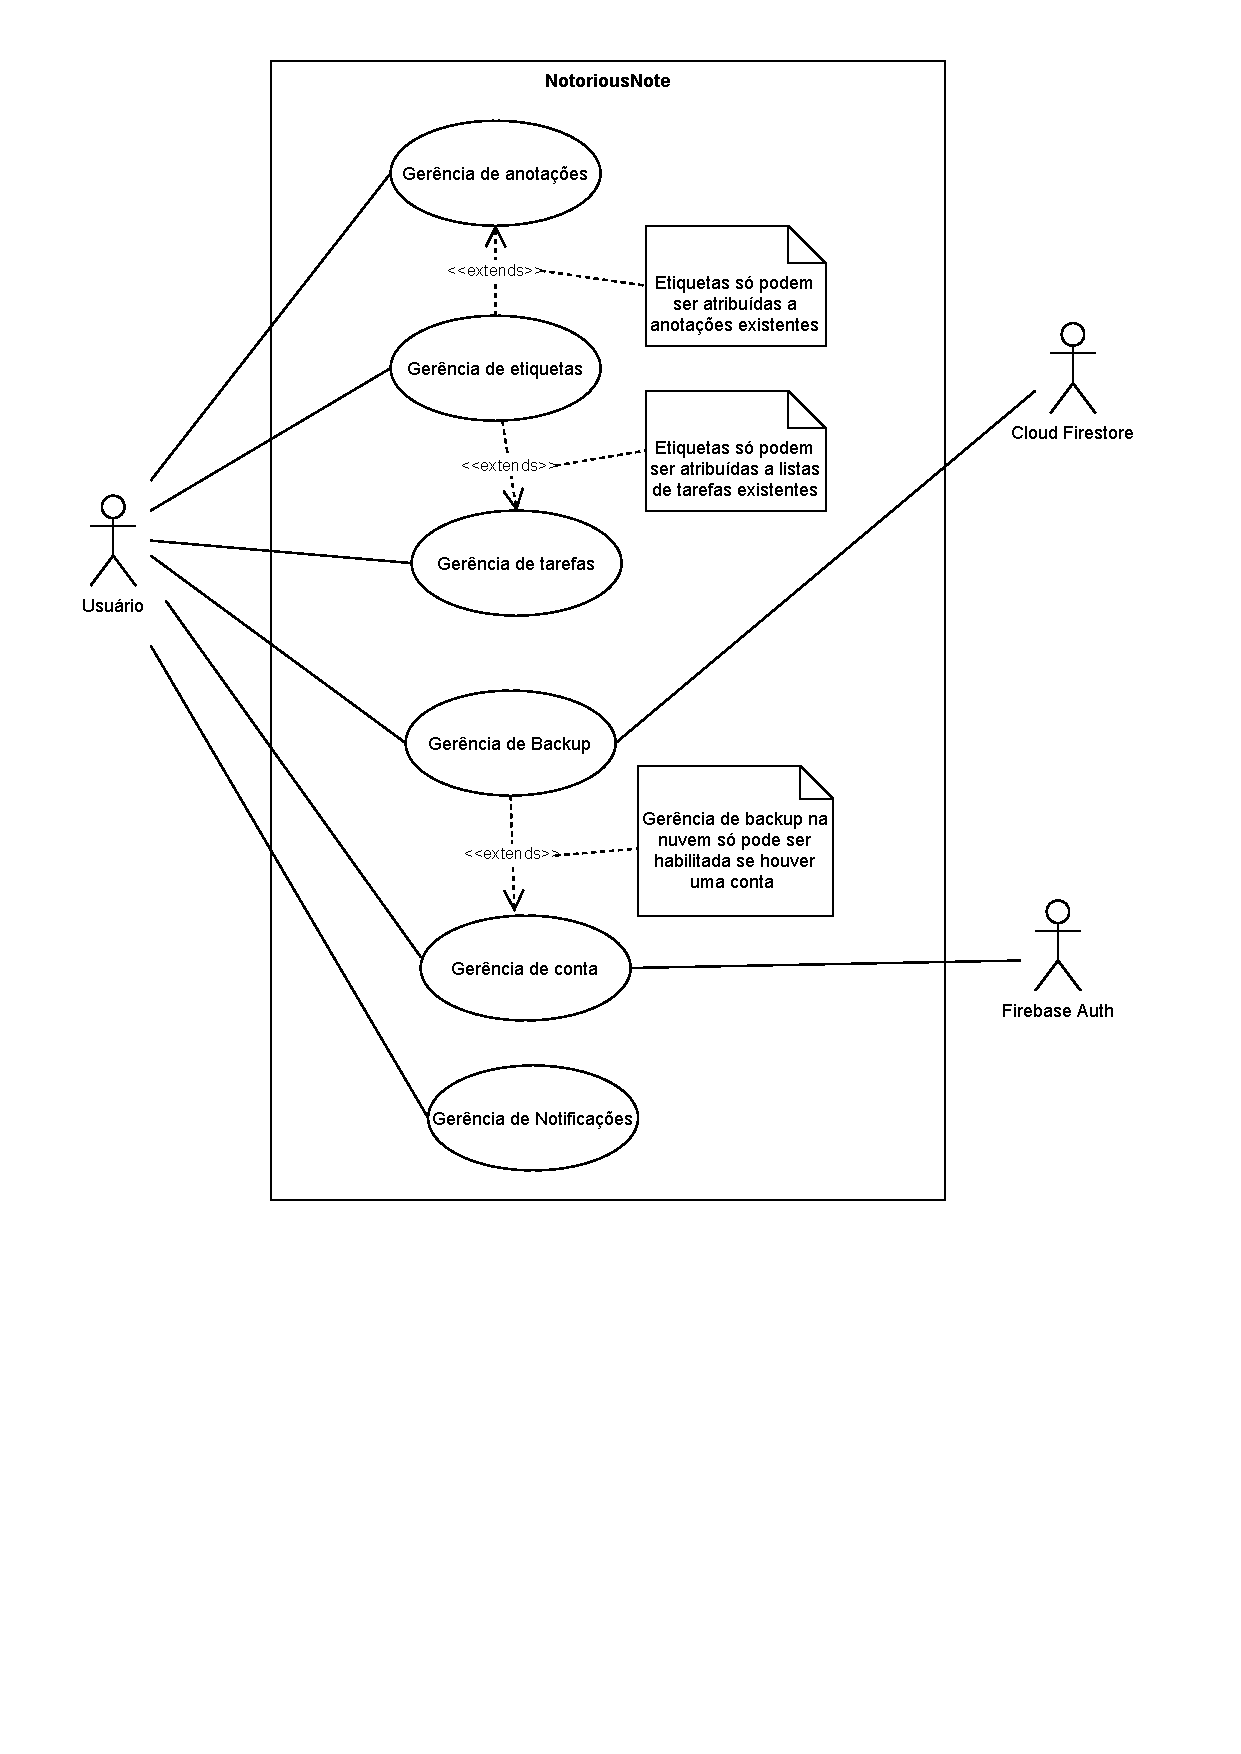
\includegraphics[keepaspectratio=true,width=\textwidth,clip=true,trim=1cm 9cm 2cm 1cm]{notoriousnote-casos-de-uso.pdf}
    \caption{Diagrama de casos de uso do sistema}
    \label{fig:diagrama_casos_uso}
\end{figure}

% \chapter{Lições Aprendidas}
%[Liste as lições aprendidas na retrospectiva, com ênfase especial nas ações a serem tomadas para melhorar, por exemplo: o ambiente de desenvolvimento, o processo ou a colaboração da equipe.]

% ----------------------------------------------------------
% Capitulo com exemplos de comandos inseridos de arquivo externo
% ----------------------------------------------------------

% ---
% Este capítulo, utilizado por diferentes exemplos do abnTeX2, ilustra o uso de
% comandos do abnTeX2 e de LaTeX.
% ---

% \include{abntex2-modelo-include-comandos}

% ----------------------------------------------------------
% Parte de resultados
% ----------------------------------------------------------
% \part{Resultados}

% ---
% Capitulo de revisão de literatura
% ---
% \chapter{Lorem ipsum dolor sit amet}

% ---
% \section{Aliquam vestibulum fringilla lorem}
% ---

% \lipsum[1]

% \lipsum[2-3]

% ---
% Finaliza a parte no bookmark do PDF
% para que se inicie o bookmark na raiz
% e adiciona espaço de parte no Sumário
% ---
\phantompart

% ---
% Conclusão
% ---
% \chapter{Conclusão}
% ---

% \lipsum[31-33]

% ----------------------------------------------------------
% ELEMENTOS PÓS-TEXTUAIS
% ----------------------------------------------------------
\postextual

% ----------------------------------------------------------
% Referências bibliográficas
% ----------------------------------------------------------
%[Listar as referências utilizadas neste documento]
\bibliography{referencias_visao.bib}

% ----------------------------------------------------------
% Glossário
% ----------------------------------------------------------
%
% Consulte o manual da classe abntex2 para orientações sobre o glossário.
%
%\glossary

% ----------------------------------------------------------
% Apêndices
% ----------------------------------------------------------

% ---
% Inicia os apêndices
% ---
% \begin{apendicesenv}

% Imprime uma página indicando o início dos apêndices
% \partapendices

% ----------------------------------------------------------
% \chapter{Quisque libero justo}
% ----------------------------------------------------------

% \lipsum[50]

% ----------------------------------------------------------
% \chapter{Nullam elementum urna vel imperdiet sodales elit ipsum pharetra ligula
% ac pretium ante justo a nulla curabitur tristique arcu eu metus}
% ----------------------------------------------------------
% \lipsum[55-57]

% \end{apendicesenv}
% ---


% ----------------------------------------------------------
% Anexos
% ----------------------------------------------------------

% ---
% Inicia os anexos
% ---
% \begin{anexosenv}

% Imprime uma página indicando o início dos anexos
% \partanexos

% ---
% \chapter{Morbi ultrices rutrum lorem.}
% ---
% \lipsum[30]

% ---
% \chapter{Cras non urna sed feugiat cum sociis natoque penatibus et magnis dis
% parturient montes nascetur ridiculus mus}
% ---

% \lipsum[31]

% ---
% \chapter{Fusce facilisis lacinia dui}
% ---

% \lipsum[32]

% \end{anexosenv}

%---------------------------------------------------------------------
% INDICE REMISSIVO
%---------------------------------------------------------------------

\phantompart

\printindex

%---------------------------------------------------------------------
% Formulário de Identificação (opcional)
%---------------------------------------------------------------------
% \chapter*[Formulário de Identificação]{Formulário de Identificação}
% \addcontentsline{toc}{chapter}{Exemplo de Formulário de Identificação}
% \label{formulado-identificacao}

% Exemplo de Formulário de Identificação, compatível com o Anexo A (informativo)
% da ABNT NBR 10719:2015. Este formulário não é um anexo. Conforme definido na
% norma, ele é o último elemento pós-textual e opcional do relatório.

% \bigskip

% \begin{tabular}{|p{9cm}|p{5cm}|}
% \hline
% \multicolumn{2}{|c|}{\textbf{\large Dados do Relatório Técnico e/ou científico}}\\
% \hline
% \multirow{4}{10cm}[24pt]{Título e subtítulo}& Classificação de segurança\\
%                   & \\
%                   \cline{2-2}
%                   & No.\\
%                   & \\

% \hline
% Tipo de relatório & Data\\
% \hline
% Título do projeto/programa/plano & No.\\
% \hline
% \multicolumn{2}{|l|}{Autor(es)} \\
% \hline
% \multicolumn{2}{|l|}{Instituição executora e endereço completo} \\
% \hline
% \multicolumn{2}{|l|}{Instituição patrocinadora e endereço completo} \\
% \hline
% \multicolumn{2}{|l|}{Resumo}\\[3cm]
% \hline
% \multicolumn{2}{|l|}{Palavras-chave/descritores}\\
% \hline
% \multicolumn{2}{|l|}{
% Edição \hfill No. de páginas \hfill No. do volume \hfill Nº de classificação \phantom{XXXX}} \\
% \hline
% \multicolumn{2}{|l|}{
% ISSN \hfill \hfill Tiragem \hfill Preço \phantom{XXXXXXXX}} \\
% \hline
% \multicolumn{2}{|l|}{Distribuidor} \\
% \hline
% \multicolumn{2}{|l|}{Observações/notas}\\[3cm]
% \hline
% \end{tabular}

\end{document}